\section{Funktionsweise}

\begin{frame}{Funktionsweise}

\begin{figure}[ht!]
	%\centering
	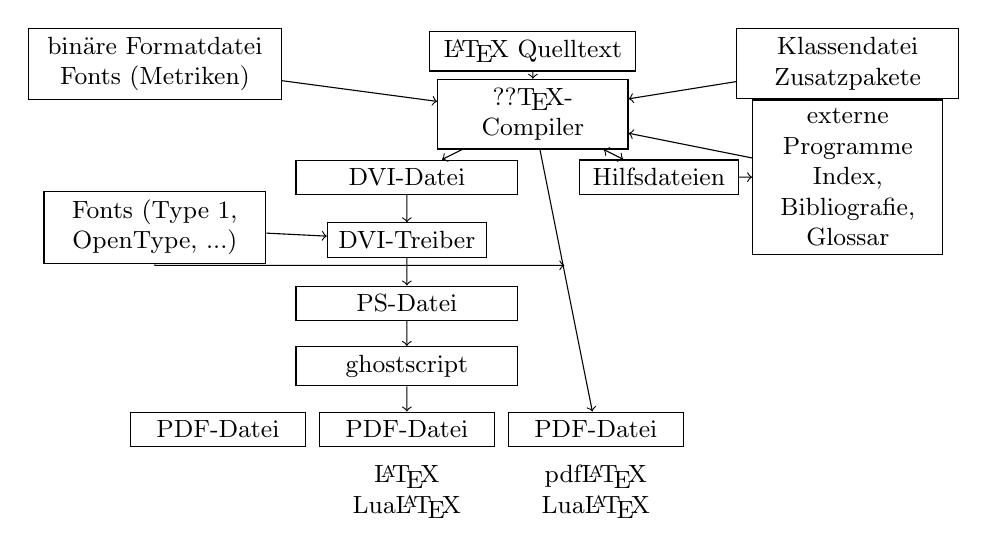
\begin{tikzpicture}[scale=0.8]
	\small
	%\centering
	\node[shape = rectangle, draw = black, text width = 2.4cm, text centered] (r1) at (8, 0) {\LaTeX{} Quelltext};
	
	\node[shape = rectangle, draw = black, text width = 2.2cm, text centered] (r2) at (8, -1) {??\TeX{}-Compiler};
	
	\node[shape = rectangle, draw = black, text width = 2.6cm, text centered] (r3) at (6, -2) {DVI-Datei};
	
	\node[shape = rectangle, draw = black, text width = 1.8cm, text centered] (r4) at (6, -3) {DVI-Treiber};
	
	\node[shape = rectangle, draw = black, text width = 2.6cm, text centered] (r5) at (6, -4) {PS-Datei};
	
	\node[shape = rectangle, draw = black, text width = 2.6cm, text centered] (r6) at (6, -5) {ghostscript};
	
	\node[shape = rectangle, draw = black, text width = 2.0cm, text centered] (r7) at (3, -6) {PDF-Datei};
	
	\node[shape = rectangle, draw = black, text width = 2.0cm, text centered] (r8) at (6, -6) {PDF-Datei};
	
	\node[shape = rectangle, draw = black, text width = 2.0cm, text centered] (r9) at (9, -6) {PDF-Datei};
	
	\node[shape = rectangle, draw = white, text width = 2.6cm, text centered](r10) at (3, -7){\XeLaTeX};
	
	\node[shape = rectangle, draw = white, text width = 2.6cm, text centered](r11) at (6, -7){\LaTeX{} \\ Lua\LaTeX{}};
	
	\node[shape = rectangle, draw = white, text width = 2.6cm, text centered](r12) at (9, -7){pdf\LaTeX{} \\ Lua\LaTeX{} \\ \XeLaTeX{}};
	
	\node[shape = rectangle, draw = black, text width = 1.8cm, text centered] (r13) at (10, -2) {Hilfsdateien};
	
	\node[shape = rectangle, draw = black, text width = 2.2cm, text centered] (r14) at (13, -2.0) {externe Programme \\ Index, \\ Bibliografie, \\ Glossar};
	
	\node[shape = rectangle, draw = black, text width = 2.6cm, text centered] (r15) at (13, -0.2) {Klassendatei \\ Zusatzpakete};
	
	\node[shape = rectangle, draw = black, text width = 3cm, text centered] (r16) at (2, -0.2) {binäre Formatdatei \\ Fonts (Metriken)};
	
	\node[shape = rectangle, draw = black, text width = 2.6cm, text centered] (r17) at (2, -2.8) {Fonts (Type 1, \\ OpenType, ...)};
	
	%\node[shape = rectangle, text centered, label = below:Start] (t1) at (0, -4) {};
	
	%\node[shape = rectangle, draw = black, text centered, fill = black, label = below:Ende] (t3) at (12, -4) {};
	
	%\node[shape = rectangle, text width = 2.5cm, text centered] (t2) at (4, -4) {Erstelle neue Population};
		
	\path[->] (r1) edge (r2);
	
	\path[->] (r2) edge (r3);
	
	\path[->] (r3) edge (r4);
	
	\path[->] (r4) edge (r5);
	
	\path[->] (r5) edge (r6);

	\path[->] (r6) edge (r8);
	
	\path[->] (r2) edge (r9);
	
	\path[->] (r15) edge (r2);
	
	\path[<->] (r13) edge (r2);
	
	\path[->] (r13) edge (r14);
	
	\path[->] (r14) edge (r2);
	
	\path[->] (r16) edge (r2);
	
	\path[->] (r17) edge (r4);
	
	\path[draw, ->] (r17) --++ (0, -0.6cm) --++ (6.5cm, 0); 
		
	%\path[->] (e1) edge node[below] {ja} (r3);
	
	%\path[->] (t1) edge (r1);
	
	%\path[->] (e1) edge node[right] {nein} (r4);
	
	%\path[->] (r3) edge (t3);
	
	%\path[->] (r4) edge (t2);
	
	%\path[->] (t2) edge (r2);
	
	\end{tikzpicture}
	\caption[Schematischer Ablauf evolution\"{a}rer Algorithmen]{Von der Quelle bis zur Mündung ...} 
	%\label{fig:processga}
\end{figure}
\end{frame}

\begin{frame}{Funktionsweise}
Für einfache Texte gelten folgende Schritte:
\begin{enumerate}
	\item Texte im Editor schreiben, bspw. mit \textit{Kile}: \texttt{kile meinText.tex}
	\item Dokument übersetzen, bspw. mit pdf\LaTeX{}: \texttt{pdflatex meinText.tex}
\end{enumerate}
Es werden dabei mindestens folgende Dateien erzeugt: \\
\begin{tabular}[pos]{lp{8.5cm}}
	\texttt{meinText.log} & Enthält alle Statusmeldungen des Übersetzungsvorgangs. \\
	\texttt{meinText.aux} & Enthält unter anderem die Einträge für Querverweise. \\
	\texttt{meinText.pdf} & Das erzeugte PDF-Dokument (nach dem ersten Durchlauf ohne Inhaltsverzeichnis).
\end{tabular}
\begin{enumerate}
	\item[3.] Erneutes Übersetzen des Dokuments: \texttt{pdflatex meinText.tex}
	\item[4.] PDF-Dokument ansehen, bspw. mit dem PDF-Viewer \textit{okular}: \texttt{okular meinText.pdf}
\end{enumerate}
\end{frame}
